% generated by plots/fig8_reasoning.py --- do not edit the numbers by hand
% figure* --- the chapter is two-column and this does not fit one
\begin{figure}[tp]
\centering
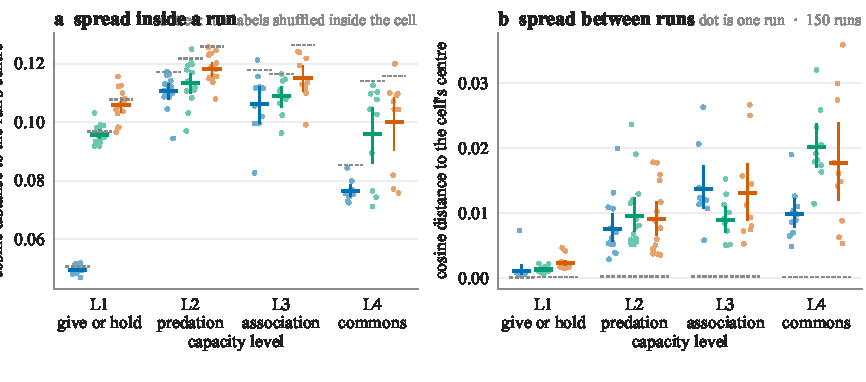
\includegraphics[width=\linewidth]{figures/fig8_reasoning/dispersion.pdf}\\[2pt]
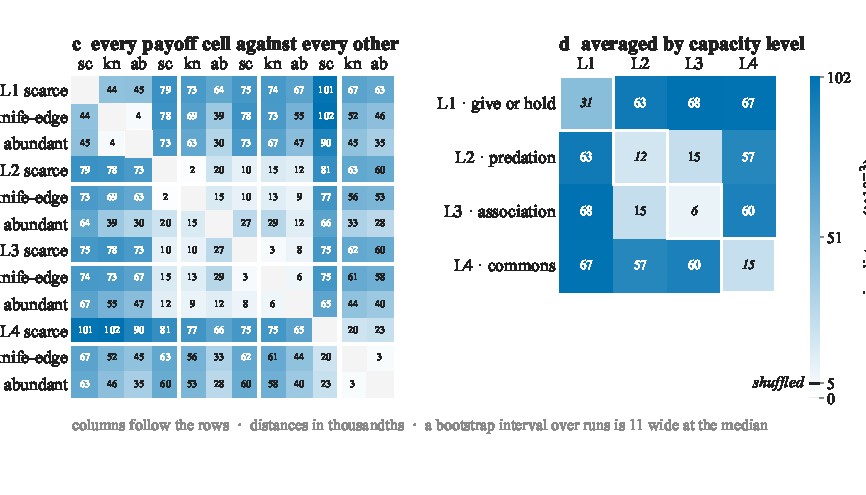
\includegraphics[width=\linewidth]{figures/fig8_reasoning/matrix.pdf}\\[2pt]
\caption[Reasoning traces in embedding space]{%
\textbf{Reasoning traces in embedding space.} How alike the reasoning of the twelve payoff cells is, read off the text the agents wrote while deciding. \textbf{(a, b)} The spread of a cell split in two, in cosine distance: how far a run's traces sit from that run's centre, and how far each run's centre sits from its cell's. A dot is one of the 150 runs, the bar is the cell mean with a 95\% interval, and the dotted rule is the same quantity with the run labels shuffled. \textbf{(c, d)} Cosine distance between the twelve cell centres, in thousandths; (d) averages by capacity level. An interval is 11 wide at the median, so a diagonal block reads as one block.}
\label{fig:reasoning}
\end{figure}
